% vim:set number:
\documentclass{book}
\usepackage[american]{circuitikz}
\usetikzlibrary{arrows.meta}

\tikzset{%
    sec/.style={line width = 0.5pt},
    blo/.style={rectangle,fill=white, inner sep=1.5pt},
    pri/.style={line width = 1pt},
    pra/.style={line width = 1pt, -{Stealth[scale width=0.7]}}
}


\begin{document}

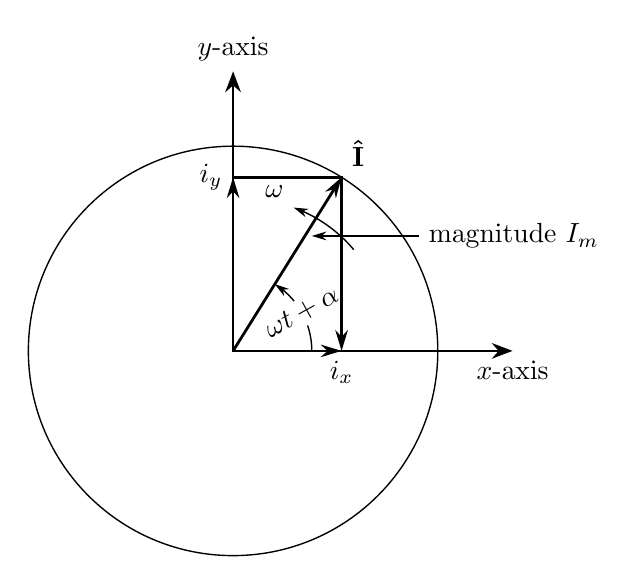
\begin{tikzpicture}[line width=1pt,-{Stealth[scale width=0.8]}]
    \coordinate (A) at (58:2.6);
    \coordinate (O) at (0,0);
    \draw [sec] (O) +(0:1)arc(0:58:1)node[blo,midway,rotate=29]{$\omega t + \alpha$};
    \draw [line width = 0.5pt](0,0)ellipse[radius=2.6];
    \draw [Stealth-Stealth](0,3.55)node [anchor = south]{$y$-axis}--(0,0)--(3.55,0)node[anchor = north]{$x$-axis};
    \draw (0,0)--(A)node[anchor=south west]{$\mathbf{\hat I}$};
    \draw [](O|-A)--(A)--(A|-O);
    \draw (O)--(O|-A)node[anchor = east]{$i_y$};
    \draw (O)--(A|-O)node[anchor = north]{$i_x$};
    \draw [sec] (O)+(40:2)arc(40:70:1.8cm)node[anchor = south east]{$\omega$};
    \draw [sec] (2.36,1.46)node[anchor = west]{magnitude $I_m$} -- (1,1.46);
\end{tikzpicture}

%-----------------------------------
%          Figura 1.2
%-----------------------------------

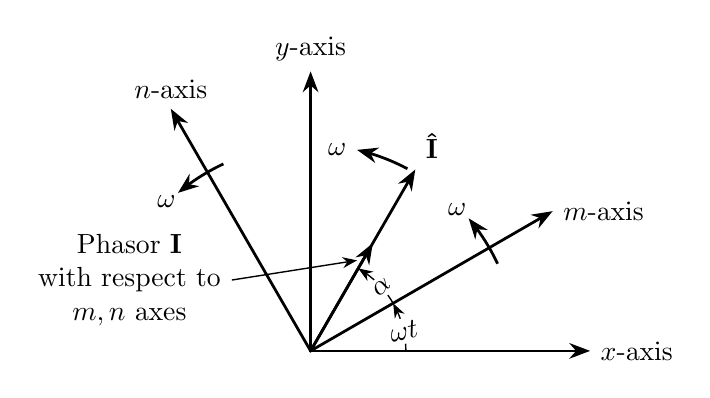
\begin{tikzpicture}[line width=1pt,-Stealth]
    \coordinate (O) at (0,0);
    \draw [Stealth-Stealth](0,3.55)node [anchor = south]{$y$-axis}--(O)--(3.55,0)node[anchor = west]{$x$-axis};
    \draw [Stealth-Stealth,rotate=30](0,3.55)node [anchor = south]{$n$-axis}--(O)--(3.55,0)node[anchor = west]{$m$-axis};
    \draw [sec] (O) +(0:1.21)arc(0:30:1.21)node[blo,pos=0.4,rotate=12]{$\omega t$};
    \draw [sec] (O) +(30:1.21)arc(30:60:1.21)node[blo,pos=0.4,rotate=42]{$\alpha$};
    \draw (O) -- (60:2.66)node[anchor = south west]{$\mathbf{\hat I}$};
    \draw (O) -- (60:1.58);
    \draw (O) +(25:2.62) arc (25:40:2.62) node[above left=-3pt]{$\omega$};
    \draw (O) +(62:2.62) arc (62:77:2.62) node[left]{$\omega$};
    \draw (O) +(115:2.62) arc (115:130:2.62) node[below left=-3pt]{$\omega$};
    \draw [sec](-1,0.9)node[text width=2.35cm,align=center,left]{Phasor $\mathbf{I}$ \\ with respect to \\$m,n$ axes}--(0.59,1.15);
\end{tikzpicture}

%-----------------------------------
%          Figura 1.3
%-----------------------------------
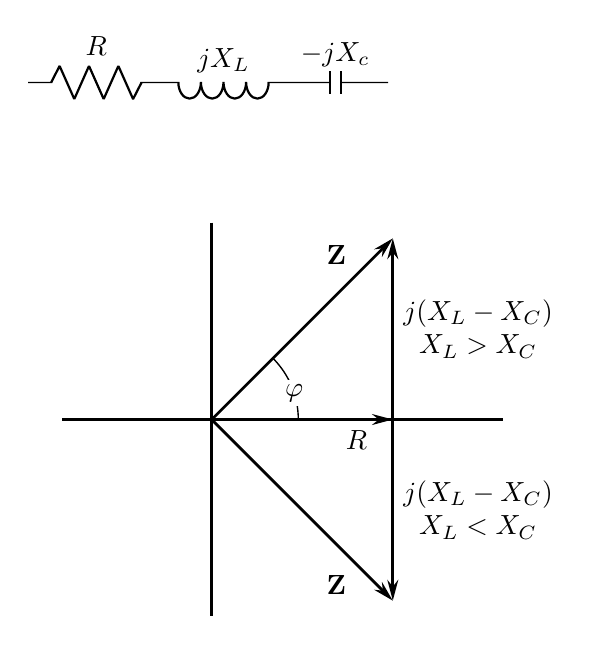
\begin{tikzpicture} %TODO corregir capacitor
    \coordinate (O) at (0,0);
    \ctikzset {bipoles/capacitor/height=0.2,bipoles/capacitor/width=0.1}
    \draw (-2.33,4.28) to[R=$R$](-0.6,4.28) (0.9,4.28)to[L,l_=$jX_L$](-0.6,4.28) (0.9,4.28)to[C=$-jX_c$](2.24,4.28);
    \draw [pri](-1.9,0)--(3.7,0) (0,2.5) -- (0,-2.5);
    \draw [pra](O)--(2.3,2.3)node[pos=0.8,above left]{$\mathbf{Z}$};
    \draw [pra](O)--(2.3,-2.3)node[pos=0.8,below left]{$\mathbf{Z}$};
    \draw [pra](O)--(2.3,0)node[pos=0.8,below]{$R$};
    \draw [pra](2.3,0)--(2.3,2.3)node[pos=0.5,right,align=center]{$j(X_L-X_C)$\\$X_L>X_C$};
    \draw [pra](2.3,0)--(2.3,-2.3)node[pos=0.5,right,align=center]{$j(X_L-X_C)$\\$X_L<X_C$};;
    \draw [sec](O) +(0:1.1)arc(0:45:1.1)node[blo,pos=0.4]{$\varphi$};
\end{tikzpicture}

%-----------------------------------
%          Figura 1.4
%-----------------------------------
\begin{tikzpicture}

\end{tikzpicture}

\end{document}
